\documentclass{beamer}
\usepackage{subfig}
\usepackage{amsmath}
\usepackage{bm}

\DeclareMathOperator*{\argmax}{arg\,max}
\DeclareMathOperator*{\argmin}{arg\,min}


\title{Neural Networks}
\author{Prof. Alessandro Lucantonio}
\institute{Aarhus University - Department of Mechanical and Production Engineering}
\date{?/?/2023}

\begin{document}
	\frame{\titlepage}
	
	\begin{frame}
		\frametitle{Motivations}
		\begin{itemize}
			\setlength\itemsep{5mm}
			\item Neural Networks (NN) are one of the most flexible ML tools.
			\item Universal approximators!
			\item Can manipulate real and discrete data $\leadsto$ regression and classification problems.
			\item Not a single model: many type of NN (e.g. MLP, CNN, RNN).
			\item Inspired by biological systems.
		\end{itemize}
	\end{frame}

	\begin{frame}
		\frametitle{Perceptron - Visualization}
		\begin{figure}
			\centering
			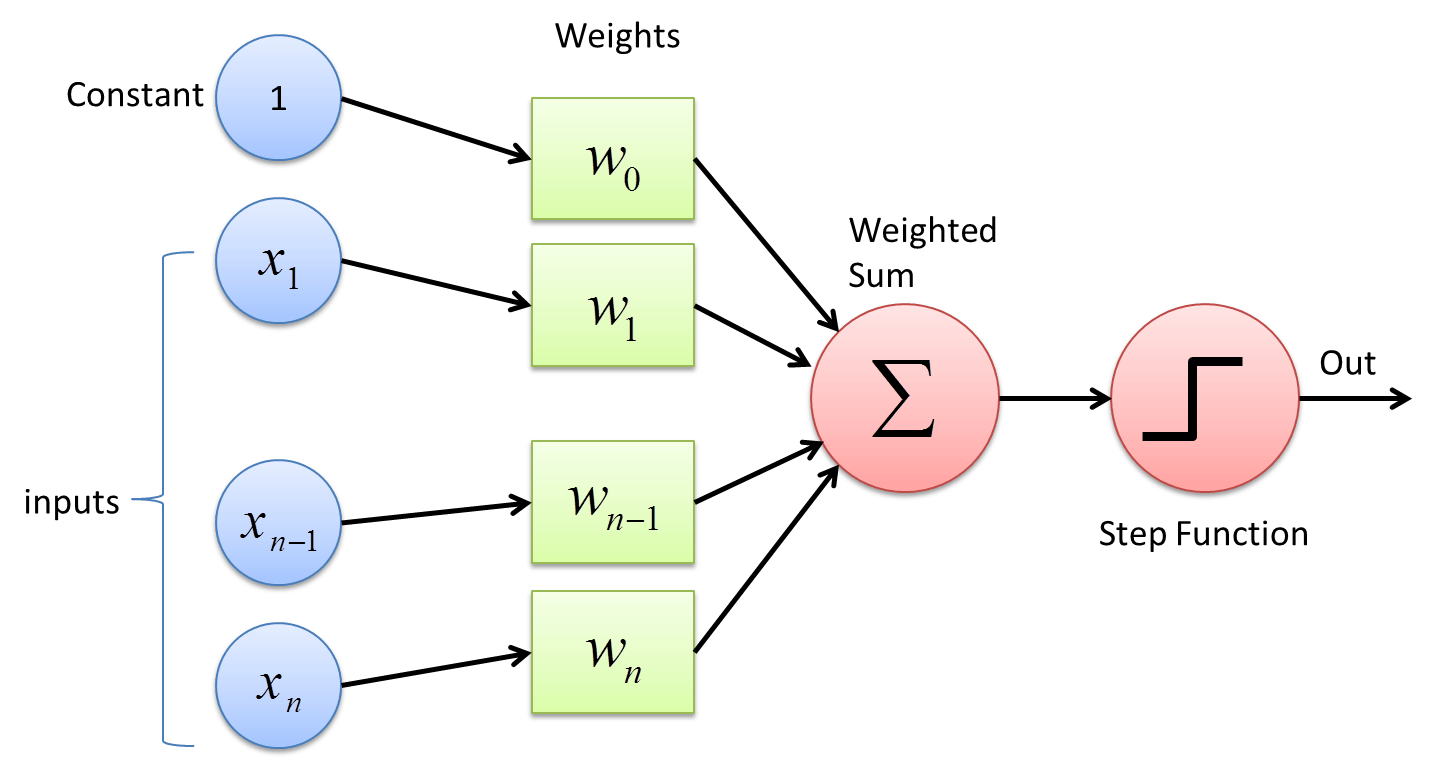
\includegraphics[scale=0.2]{images/perceptron}
			\caption{Representation of a perceptron.}
		\end{figure}
	\end{frame}

	\begin{frame}
		\frametitle{Perceptron - Formal}
		Notation: $n$ is as usual the number of features. $x$ is an input sample of length $n+1$ with $x_0 = 1$.
		
		\vspace{5mm}
		
		Perceptron:
		\begin{equation*}
			\begin{cases}
				n(\bm{x}) := \bm{w}^T \bm{x} = \sum_{j=0}^{n} w_j x_j,\\
				h(\bm{x}) := f(n(\bm{x})).
			\end{cases}
		\end{equation*}
	
		$n$ is the \textbf{net input} to the neuron.
		
		\vspace{5mm}
		
		$f$ is called \textbf{activation function}. Some common examples are:
		\begin{itemize}
			\item Linear:  $f(t) = at + b$.
			\item ReLU (Rectified Linear Unit): $f(t) := \max\{0, t\}$.
			\item Sigmoid: $f(t) := \frac{1}{1 + e^{-t}}$.
			\item Tanh (Hyperbolic tangent): $f(t) := \frac{e^{2t}-1}{e^{2t}+1}$
		\end{itemize}
		
	\end{frame}
	
	\begin{frame}
		\frametitle{Activation Functions - Visualization}
		\begin{figure}
			\centering
			\subfloat[Linear]{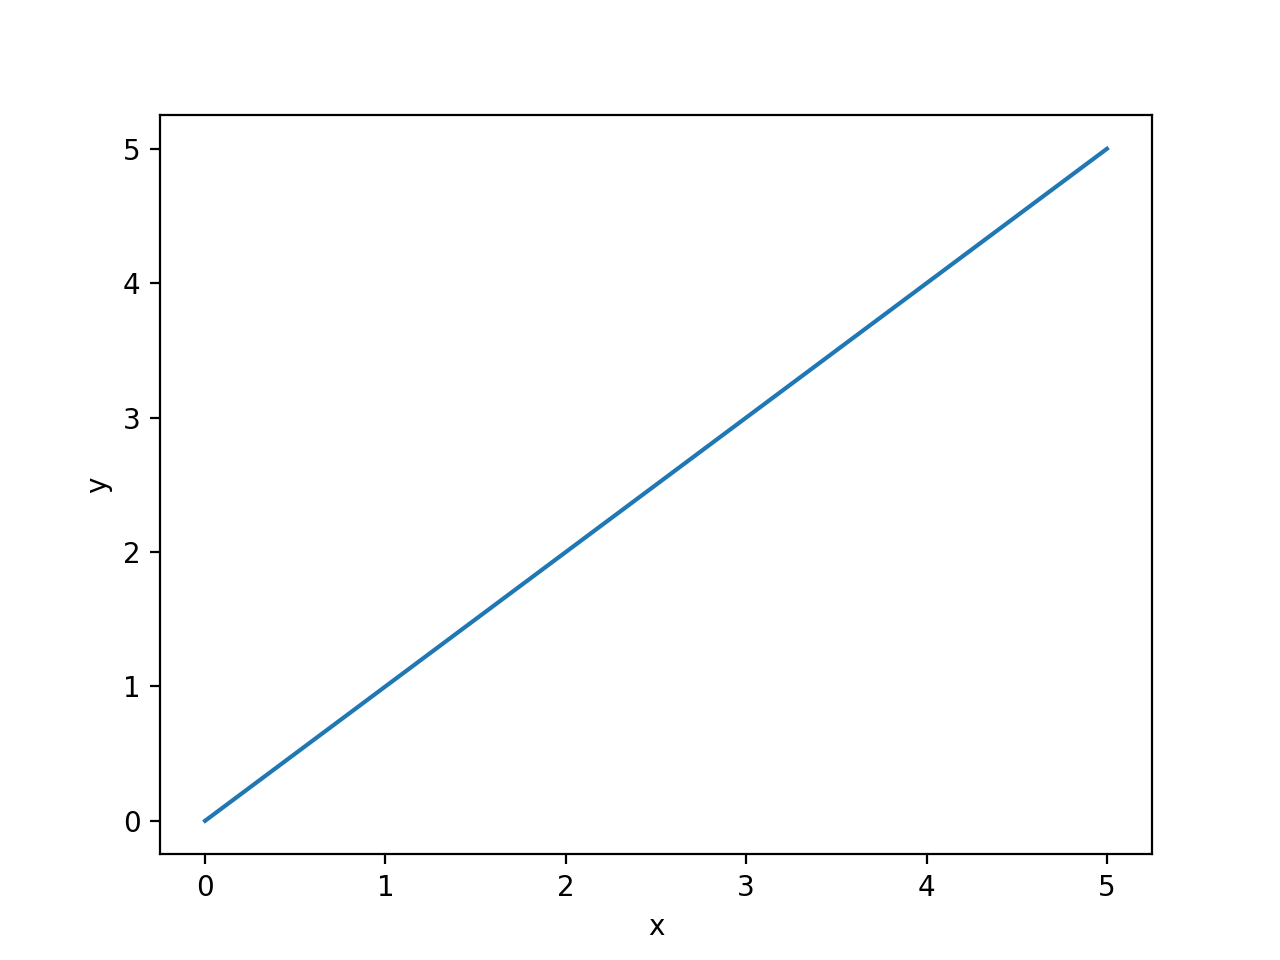
\includegraphics[scale=0.25]{images/linear}}
			\qquad
			\subfloat[ReLU]{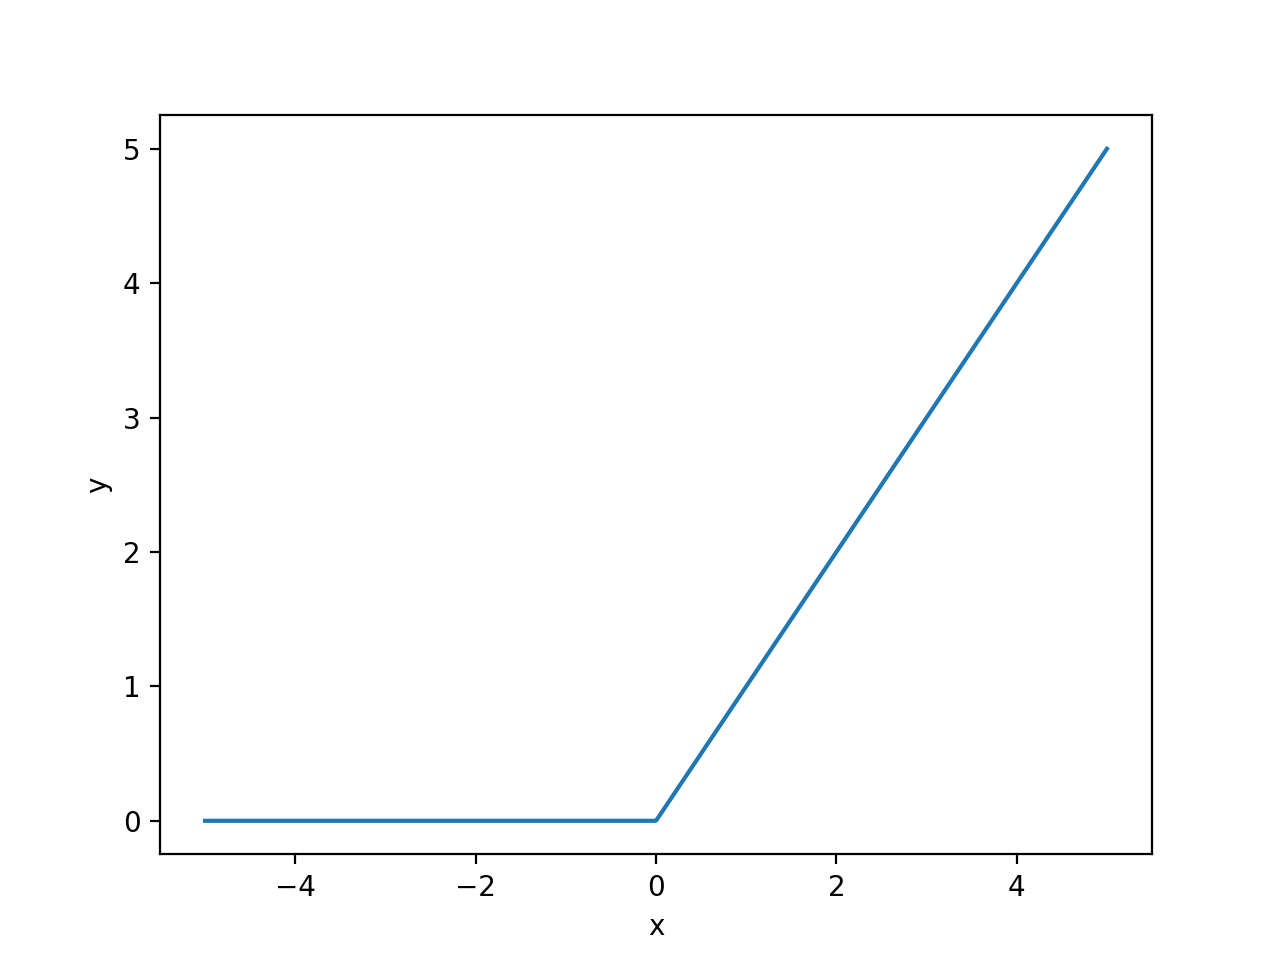
\includegraphics[scale=0.25]{images/relu}}
			\\ \vspace{0.1cm}
			\subfloat[Sigmoid]{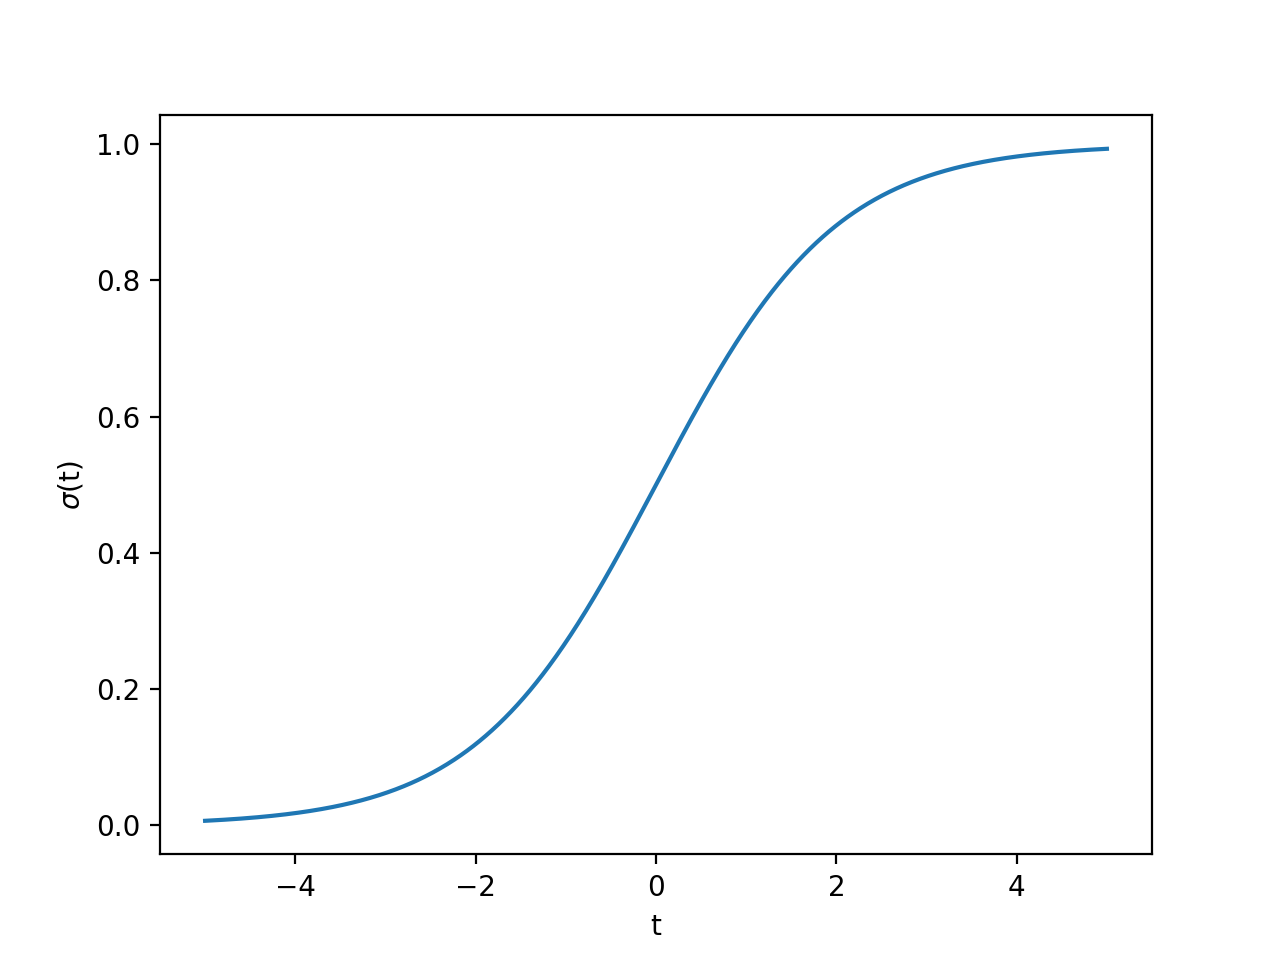
\includegraphics[scale=0.25]{images/sigmoid}}
			\qquad
			\subfloat[Tanh]{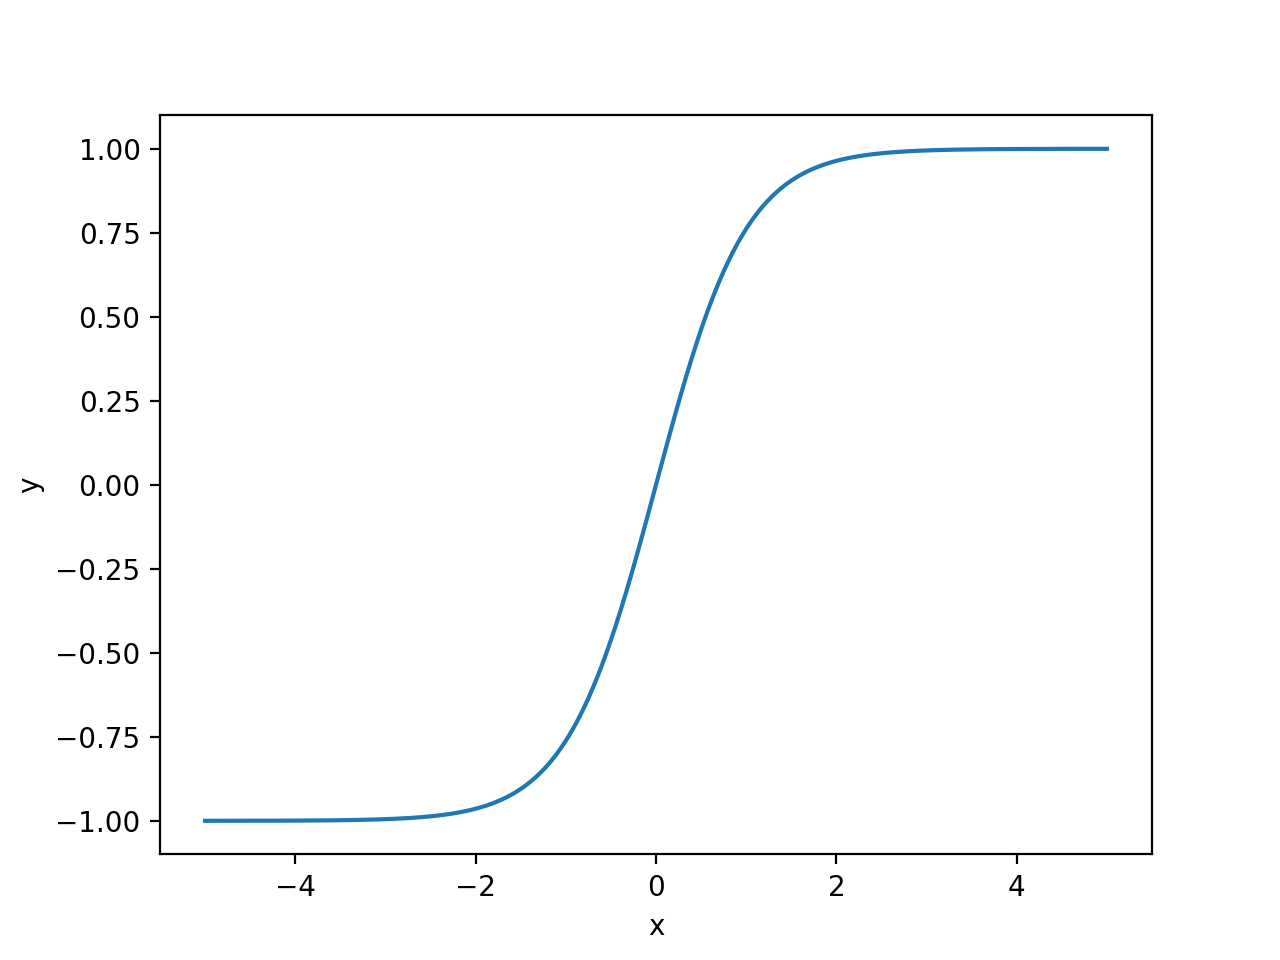
\includegraphics[scale=0.25]{images/tanh}}
		\end{figure}
	\end{frame}

	\begin{frame}
		\frametitle{MultiLayer Perceptron (MLP) - Visualization}
		\begin{figure}
			\centering
			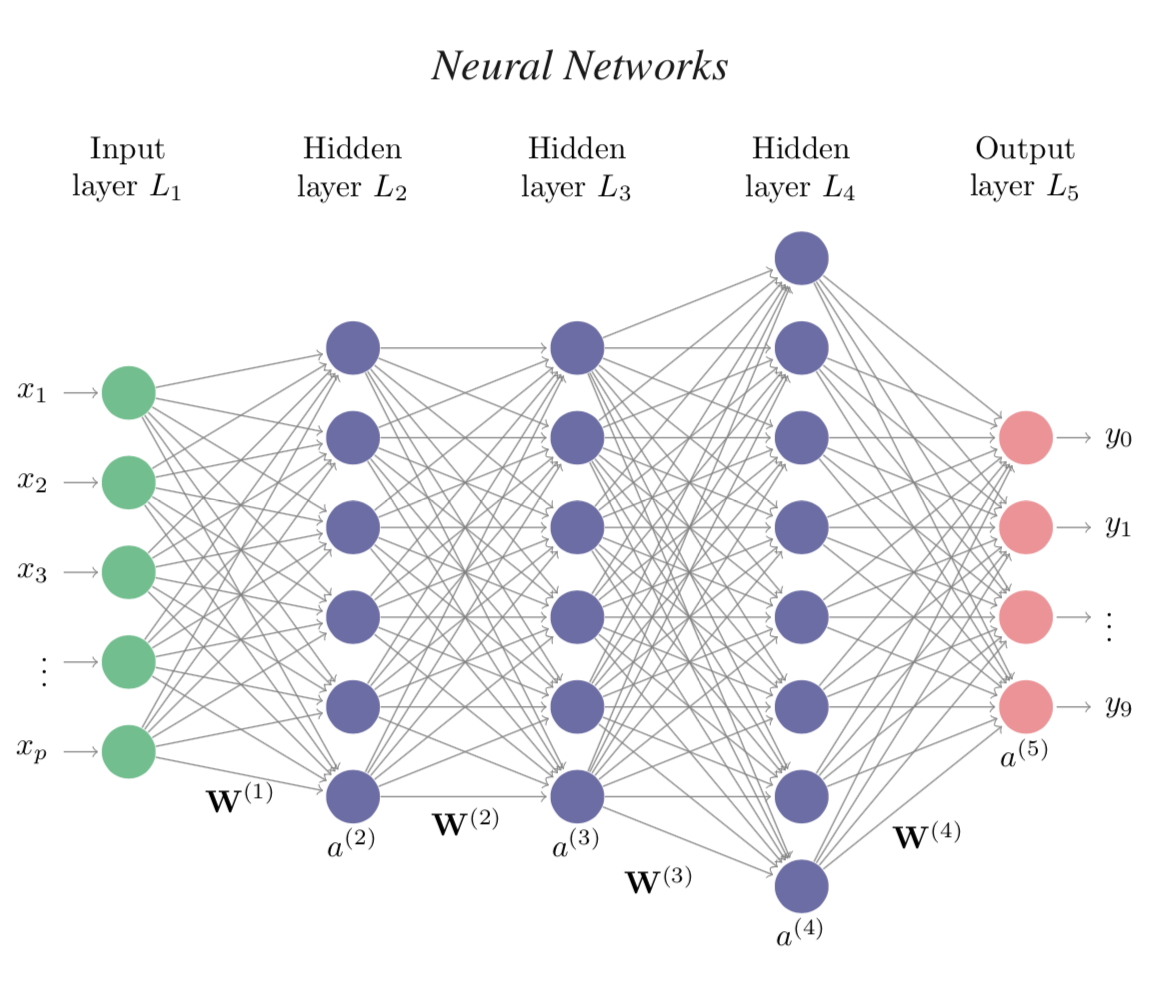
\includegraphics[scale=0.23]{images/mlp}
		\end{figure}
	\end{frame}

	\begin{frame}
		\frametitle{MLP - Formal}
		Notation: $\bm{a}^{(i)}$ is the input vector of the $i$-th layer and $\mathsf{W}^{(i)}$ is the weight matrix for each layer. $m$ is the number of layers.
		
		\vspace{5mm}
		
		Parenthesis: Why do we have a weight matrix for each layer? Each layer $i$ consists of $m_i$ neurons, hence necessarily has $m_i$ weight vectors, which we can arrange row-wise to form the matrix $\mathsf{W}^{(i)}$.
		
		\vspace{5mm} 
		
		For each layer $i$ compute
		\begin{equation*}
			\begin{cases}
				n_i(\bm{a}^{(i)}) := \mathsf{W}^{(i)} \bm{a}^{(i)},\\
				h_i(\bm{a}^{(i)}) := f_i(n_i(\bm{a}^{(i)})).
			\end{cases}
		\end{equation*}
	Compact form:
	\begin{equation*}
		h(\bm{x}) := f_{m-1}\big(\mathsf{W}^{(m-1)}f_{m-2}\big(\cdots f_1 \big(\mathsf{W}^{(1)} \bm{x}\big) \cdots\big)\big)
	\end{equation*}
	\end{frame}

	\begin{frame}
		\frametitle{MLP - Some comments}
		\begin{itemize}
			\setlength\itemsep{5mm}
			\item This kind of NN are also called \textbf{feedforward NN}, since we transfer information from input to output.
			\item The hypothesis function is non-convex! This is due to the fact that composition of convex functions is not necessarily convex. Hence, in the learning problem we will have many local minima and saddle points.
			\item Theory tells us that MLP with just $1$ hidden layer are universal approximators, in the sense that they approximate as well as you want "each" continuous function (not a formal statement, just to provide intuition).
		\end{itemize}
	\end{frame}

	\begin{frame}
		\frametitle{Tips and Tricks - Is one layer really enough?}
		Theory suggests us that the answer is yes, but pay attention. There exists cases for which an exponential number of units (w.r.t. the input dimension) are required to approximate well the data.
		
		\vspace{5mm}
		
		Introducing many layers helps to reduce the total number of units but complicate a bit the learning procedure (see later).
		
		\vspace{5mm}
		
		Then the question becomes: how to find the optimal number of layers? Validation is your best friend :)
		
		Include in your model selection process as many different architectures/activation functions as you can.
	\end{frame}
\end{document}